\documentclass[12pt]{report}
\usepackage{datetime2}
\renewcommand{\baselinestretch}{1.2} 
\usepackage[breaklinks]{hyperref}
\hypersetup{
    colorlinks,%
    citecolor=black,%
    filecolor=black,%
    linkcolor=black,%
    urlcolor=cyan
}
\author{Harshad}
\usepackage{listings}
\usepackage{mathpazo}
\usepackage{amsmath}
\usepackage{amssymb}
\usepackage{amsfonts}
\usepackage[utf8]{inputenc}
\usepackage[title,titletoc]{appendix}
\usepackage{listings}
\usepackage{graphicx,enumerate,bigints}
\usepackage{amsmath,mathtools}
\usepackage{subfig,morefloats}
\usepackage{epstopdf}
\usepackage{geometry}
\geometry{verbose,tmargin=3cm,bmargin=3cm,lmargin=2.8cm,rmargin=2.8cm}
\setcounter{secnumdepth}{3}
\setcounter{tocdepth}{3}
\usepackage{graphicx,enumerate}
\usepackage{amsmath}
\usepackage{array}
\usepackage{tabularx}
\usepackage{gensymb}
\usepackage{nicefrac}
\usepackage{color}
\usepackage{algorithm}
\usepackage{algpseudocode}
\makeatletter
\providecommand{\tabularnewline}{\\}
\makeatother
 \usepackage[normalem]{ulem}
 \useunder{\uline}{\ul}{}
  \usepackage{multirow}
% \usepackage[normalem]{ulem}
% \useunder{\uline}{\ul}{}

\usepackage{subfig,morefloats}
\usepackage{booktabs}
\usepackage{fancyhdr}
\usepackage{float}
\usepackage{lastpage}
\usepackage{textcomp}
\definecolor{codegreen}{rgb}{0,0.6,0}
\definecolor{codegray}{rgb}{0.5,0.5,0.5}
\definecolor{codepurple}{rgb}{0.58,0,0.82}
\definecolor{backcolour}{rgb}{0.95,0.95,0.92}

\lstdefinestyle{mystyle}{
    backgroundcolor=\color{backcolour},   
    commentstyle=\color{codegreen},
    keywordstyle=\color{magenta},
    numberstyle=\tiny\color{codegray},
    stringstyle=\color{codepurple},
    basicstyle=\ttfamily\footnotesize,
    breakatwhitespace=false,         
    breaklines=true,                 
    captionpos=b,                    
    keepspaces=true,                 
    numbers=left,                    
    numbersep=5pt,                  
    showspaces=false,                
    showstringspaces=false,
    showtabs=false,                  
    tabsize=2
}

\lstset{style=mystyle}
%\pagestyle{fancyplain}
\fancyhf{}
\newcolumntype{P}[1]{>{\centering\arraybackslash}p{#1}}

\begin{document}
\renewcommand{\arraystretch}{1.5}
\begin{center}
%\vspace*{30pt}
\Large
\textbf{Design and Development of Network Interface Subsystem for AJIT Processor-based SoC}\\
\bigskip
\bigskip
\bigskip
\large
%MTP Stage 1 Report
\textbf{Master's Thesis}\\
\bigskip
\normalsize
\vspace*{0.5cm}
Submitted in partial fulfillment of the requirements
\\for the degree of\\
\vspace*{.8cm} \textbf{Master of Technology}\\
\textbf{Integrated Circuits and Systems}\\
\vspace*{0.5cm}
by\\
\vspace*{0.5cm}
\textbf{\large Mr. Harshad Bhausaheb Ugale} \\
\textbf{Roll No. 20307R008}\\


\vspace*{0.5cm}

under the supervision of\\
\textbf{Prof. Madhav P. Desai}\\
\vspace*{1cm}


\vspace*{0.5cm}
\begin{figure}[h!]
 \centering
 
\includegraphics[width=4cm]{iitb_logo.jpg}
 % emblem.PNG: 124x134 pixel, 72dpi, 4.37x4.73 cm, bb=0 0 124 134
\end{figure}
% \bigskip
\bigskip
%\large
\textbf{Department of Electrical Engineering}\\
\bigskip
\textbf{INDIAN INSTITUTE OF TECHNOLOGY BOMBAY}\\
\textbf{Powai, Mumbai - 400076}\\
\textbf{June 2023}\\
\end{center}
\thispagestyle{empty}

%%%%%%%%%%%%%%%%%%%%%%%%%%%%%%%%%%%%%%%%%%%%%%%%%%%%%%%%%%%%%%%%%%%%%%%%%
\newpage
\pagenumbering{roman}
%%%%%%%%%%%%%%%%%%%%%%%%%%%%%%%%%%%%%%%%%%%%%%%%%%%%%%%%%%%%%%%%%%%%%%%%%
\chapter*{}
\begin{center}
{\Large \textbf{Dissertation Approval}}

\bigskip
\bigskip
\bigskip
This dissertation entitled\\
\bigskip
\textbf{Design and Development of Network Interface Subsystem for AJIT Processor-based SoC}\\
\bigskip

by\\
\bigskip

Mr. Harshad Bhausaheb Ugale\\
Roll No. 20307R008\\
\bigskip
is   approved for the degree of\\
\textbf{Master of Technology in Electrical Engineering}\\

\end{center}
 \vspace{10mm}
\begingroup
\setlength{\tabcolsep}{30pt}
\begin{center}
    \begin{tabular}{c c}
        ..................................................... & .....................................................\\
        Prof. Madhav P. Desai & Prof. Kavi Arya\\
        (Supervisor)     & (Examiner)\\
        \\\\
        ..................................................... & .....................................................\\
        Prof. Kavi Arya   & Prof. D. Manjunath\\
        (Chairman) & (Examiner)\\
    \end{tabular}
\end{center}
\endgroup
\bigskip
{Date: \today}\\
{Place: IIT Bombay}


% ------------------------------------------------------------------------------
\newpage








%%%%%%%%%%%%%%%%%%%%%%%%%%%%%%%%%%%%%%%%%%%%%%%%%%%%%%%%%%%%%%%%%%%%%%%%%
\chapter*{}
\begin{center}
{\Large \textbf{Declaration}}
\end{center}
\bigskip
\bigskip
\bigskip
I declare that this written submission represents my ideas in my own words and where
others' ideas or words have been included, I have adequately cited and referenced the sources.  
I also declare that I have adhered to all principles of academic honesty and integrity
and   have   not   misrepresented   or   fabricated   or   falsified   any   idea/data/fact/source   in   my
submission.  I understand that any violation of the above will be cause for disciplinary action
by the Institute and can also evoke  penal action from the sources which have thus not been
properly cited or from whom proper permission has not been taken when needed.\\
\bigskip
\bigskip
\bigskip
\begin{flushleft}
..................................\\
{Mr. Harshad Bhausaheb Ugale\\
Roll No. 20307R008}
\end{flushleft}

\begin{flushleft}
{Date : \today}
\end{flushleft}

% ------------------------------------------------------------------------------
\newpage

\chapter*{}
\begin{center}
{\Large \textbf{Acknowledgment}}
\end{center}
I want to express my heartfelt gratitude towards \textbf{Prof. Madhav P. Desai} for allowing to work on this project and providing her valuable guidance throughout. His suggestions have helped me in gaining a better understanding of this research topic.\\\\
I would also like to thank members of \textbf{VLSI Lab} for providing all the necessary support.\\\\
Lastly, I am perpetually thankful to my family and friends for their unwavering encouragement and support.
% --------------------------------------------------------------------------------

\newpage
\chapter*{}
\begin{center}
{\Large \textbf{Abstract}}
\end{center}
The rapid advancement of network technologies has created a growing demand for efficient and reliable network communication solutions. As a result, the integration of a Network Interface Controller (NIC) into an indigenous AJIT processor-based System-on-Chip (SoC) has become increasingly crucial. This thesis aims to address this need by designing and developing a NIC that enables seamless network connectivity and communication capabilities for the AJIT processor. Additionally, it highlights the growing reliance of AI and ML technologies on network-based applications.\\

The outcomes of this research demonstrate the successful integration of the NIC into the AJIT SoC prototype. The NIC design and verification are carried out using AHIR-V2 tools, which provide an algorithmic approach to digital design. The developed NIC empowers the AJIT processor to efficiently send and receive data packets over the network, facilitating seamless connectivity with external devices and systems. Moreover, an AI/ML inference engine is employed to showcase the potential of leveraging Ethernet interface for advanced computational tasks.\\

The implications of this research extend beyond the immediate context of the AI/ML inference engine. The designed version of the NIC is flexible and can be modified to incorporate additional complex functionalities, such as self-routing and NIC-to-NIC communication. This opens up possibilities for the development of routers and other network devices with multiple NICs, offering enhanced network capabilities.\\
\par
 
%%%%%%%%%%%%%%%%%%%%%%%%%%%%%%%%%%%%%%%%%%%%list of figures
\tableofcontents
\newpage
\listoffigures
\listoftables
%\lipsum[1-20]
%\newpage                     A three-line code for empty page insertion
%\thispagestyle{empty}
%\mbox{}



\newpage

\clearpage
\pagenumbering{arabic}




\chapter{Introduction} \label{1}
%\label{ch:intro}
\rule[10pt]{\linewidth}{3pt}
 
The rapid advancement of network technologies has revolutionized various aspects of our lives, ranging from communication to data processing and beyond. In this era of interconnected systems, the need for efficient and reliable network communication solutions has become paramount. The integration of a Network Interface Controller (NIC) into an indigenous AJIT processor-based System-on-Chip (SoC) serves as a crucial step towards achieving seamless network connectivity and communication capabilities.

This chapter provides an introduction to the design and development of a Network Interface Controller for the AJIT processor-based SoC. The AJIT processor, being an indigenous processor offers unique opportunities for customization and optimization to meet specific requirements. By integrating a NIC, the AJIT SoC can effectively send and receive data packets over the network, enabling seamless connectivity with external devices and systems. Furthermore, this chapter discusses the goals and challenges, associated with the design and development of the Network Interface Controller. The goals include integrating the Ethernet interface into the AJIT SoC prototype, demonstrating the use of an AI/ML acceleration application, and generalizing the design for network appliance SoCs such as routers. By achieving these goals, the research contributes to the broader field of network communication solutions. 

Overall, this chapter sets the stage for the subsequent chapters, which delve into the design, implementation, and evaluation of the Network Interface Controller. It establishes the importance of network connectivity in the context of the AJIT processor-based SoC and provides a roadmap for the rest of the thesis.



	\section{Objectives}

		\subsection{Integration of Ethernet into AJIT System-on-Chip (SoC) Prototype}
			The first objective is to successfully integrate an Ethernet interface into the AJIT SoC prototype. This involves designing and implementing the necessary hardware components(Network Interface Controller) and firmware to enable Ethernet connectivity.

		\subsection{Network-Accelerated AI/ML Application using Ethernet Interface}
			The second objective is to utilize the integrated Ethernet interface of the AJIT processor to enable network-accelerated execution of AI/ML acceleration applications. This demonstration highlights the synergy between the processor's advanced computing capabilities and enhanced connectivity, showcasing the seamless integration of the Ethernet interface to support efficient processing and communication in networked AI/ML workloads.

		\subsection{Generalization to Network Appliance SoC (Router)}
			The third objective aims to generalize the network interface design to a broader context by extending it to a network appliance SoC, specifically a router. This involves evaluating the feasibility of incorporating the network interface into a router SoC, considering factors such as performance, power consumption, and compatibility with networking protocols.

By achieving these goals, this research aims to enhance the AJIT processor's capabilities and explore its potential in networked computing systems, paving the way for future advancements in indigenous processor development.

	\section{Challenges}

		\subsection{Network Interface Controller Design and Validation}
   One of the key challenges in this research is the design and validation of the network interface controller. This involves designing a controller that can efficiently handle the transmission and reception of Ethernet packets, ensuring proper synchronization, error handling, and protocol compliance. The validation process includes rigorous testing to verify the functionality, performance, and reliability of the controller under different network conditions and workloads.

		\subsection{Integration of Xilinx's MAC IP}
   Another challenge is the integration and configuration of Xilinx's MAC (Media Access Controller) IP into the network interface design. This requires understanding the specifications and functionality of the MAC IP and ensuring its seamless integration with the AJIT processor's architecture. The challenge includes addressing any compatibility issues, optimizing configurations, and verifying the correct operation of the MAC IP within the overall network interface design.

		\subsection{Software Design for Reliable Exchange of Information over Ethernet}
   Implementing reliable communication over Ethernet presents a challenge that requires careful software design. This involves developing protocols and algorithms to ensure the reliable exchange of information between the AJIT processor and external devices connected via Ethernet. The software design should handle packet loss, retransmissions, flow control, and other mechanisms to guarantee the integrity and timeliness of data transmission in the networked environment.

		\subsection{Software Design for SOC Firmware in AI/ML Acceleration Application}
   In the context of the AI/ML acceleration application, a significant challenge lies in the software design of the system-on-chip (SoC) firmware. This involves developing firmware that efficiently interacts with the network interface, handles data transmission and reception, and interfaces with the AI/ML acceleration modules. The firmware should be optimized for performance, ensuring seamless integration of the AI/ML application with the Ethernet interface and leveraging the network acceleration capabilities of the AJIT processor.\\\\





	The brief description of chapter's is as follows,

	\begin{itemize}
		\item Chapter~\ref{2}. Design and Validation of Network Interface Controller : In this chapter we describe the design of the NIC in detail which is then followed by the performance.
		\item Chapter~\ref{3}. SoC Design and Validation : The integration of Ethernet sub-system and accelrator is described and results are shown.
		\item Chapter~\ref{4}. Conclusion \& Future Work : Written conclsion of the work done and what can be future work options are described.
	\end{itemize}

%\section{Background} \label{1.1}

%\section{Objective}
%%%%%%%%%%%%%%%%%%%%%%%%%%%%%%%%%%%%%%%%%%%%%%%%%%%%%%%%%%%%%%

\chapter{Design and Validation of Network Interface Controller} \label{2}
\rule[10pt]{\linewidth}{3pt}
This chapter focuses on the design and validation of the Network Interface Controller (NIC) for the AJIT processor-based System-on-Chip (SoC). The NIC plays a critical role in enabling network connectivity and communication capabilities within the SoC.

The design of the NIC involves several components and considerations, including network protocol support, data packet handling, memory management, and interface with the AJIT processor. To ensure a robust and reliable design, the NIC undergoes a rigorous validation process to verify its functionality, performance, and compatibility with the AJIT SoC architecture.

The primary goal of this chapter is to provide a detailed overview of the design process, highlighting the key components and their interconnections. It explores the challenges encountered during the design phase and discusses the solutions and design choices made to overcome them. Additionally, the chapter delves into the validation methodologies employed to ensure the correctness and efficiency of the NIC design.

By describing the design and validation of the NIC, this chapter aims to provide insights into implementing a network interface solution for the AJIT processor-based SoC. It serves as a foundation for subsequent chapters, which will explore specific aspects of the NIC design, such as the data packet handling mechanisms, and memory management schemes.

	
	\section{Design decisions}
		Before directly jumping on NIC design let's take a look at the necessary design decisions made. The NIC will receive packet data from MAC
		which will be stored in memory. The processor will need to allocate this memory and provide that information to NIC. This overall needs to
		3 main interfaces to NIC. Figure~\ref{fig:NIC-Proc-top-level} shows all the interfaces.We examine each interface in detail.	

		\begin{figure}[h]
			\centering
			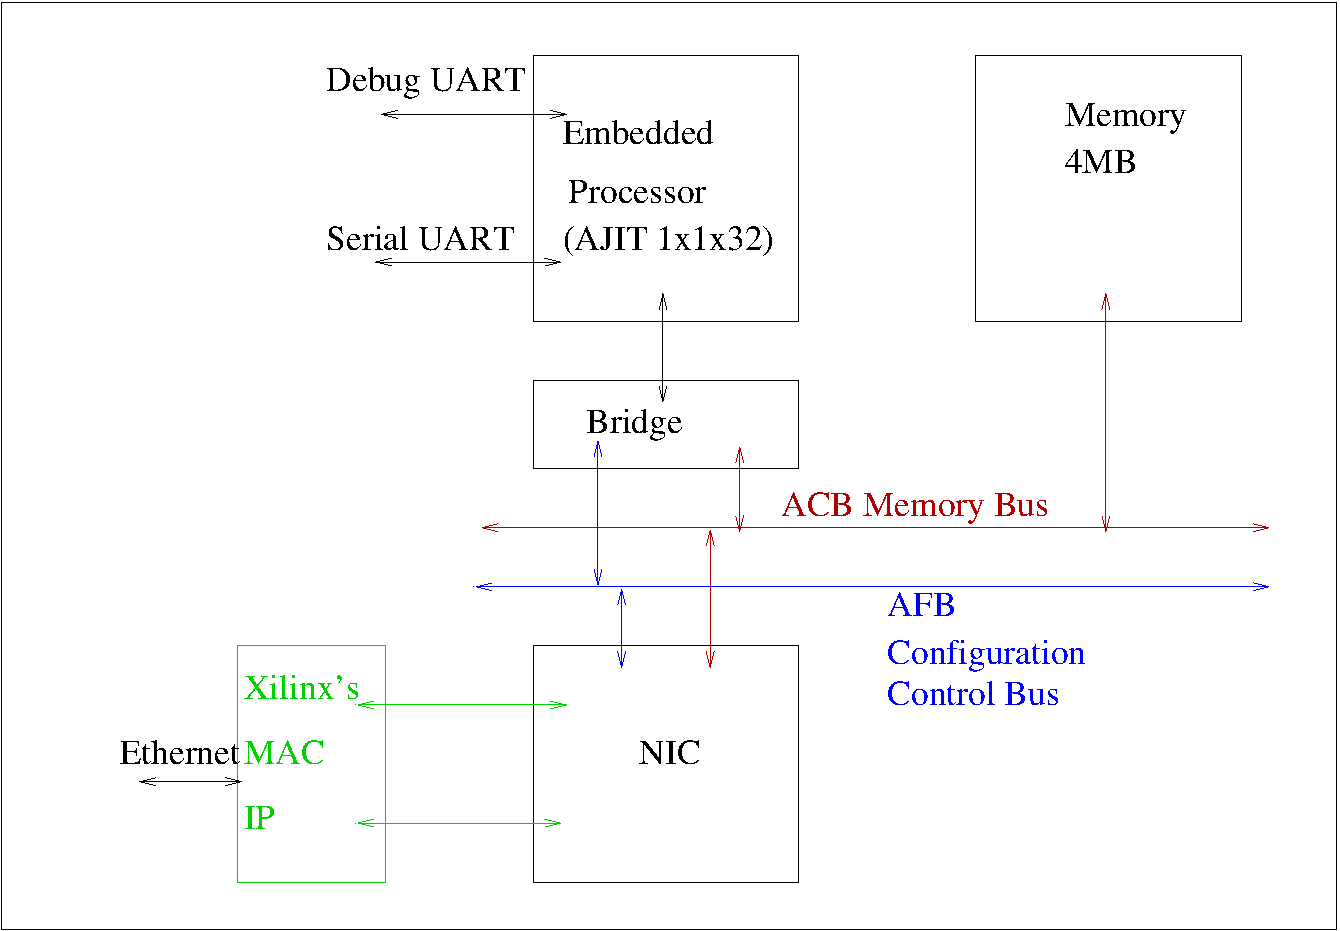
\includegraphics[width=12cm]{./figures/top_level_for_interfaces.pdf}
			\caption{Top level with Interfaces}
			\label{fig:NIC-Proc-top-level}
		\end{figure}




		\subsection{NIC-MAC interface}
			NIC to MAC interface will used by NIC for receiving and transmitting packets from MAC. The memory which will be used is provided 8 bytes per request.
			So this interface is kept 73(64 bit data + 9 bit control) bits. The bit mapping is shown in table~\ref{tab:NIC-MAC-interface}.
				\begin{table}[!htbp]
					\centering
					\begin{tabular}{ccl}
						\hline
						\textbf{Signal Name} & \textbf{Location} &\textbf{Signal Description}  \\ \hline
						\multirow{2}{*}{\textit{tlast}}	& \multirow{2}{*}{[72:72]}	& The \textit{tlast} becomes `1' if the 64 bit chunk is last\\
										& 				& chunk of packet.\\ \hline
						\textit{tdata}   		& [71: 8] 			& The \textit{tdata} is actual packet data chunk.\\ \hline
						\multirow{3}{*}{\textit{tkeep}}	& \multirow{3}{*}{[ 7: 0]}	& The \textit{tkeep} is 8 bit field, each bit is mapped\\
										&				& to 8 bytes of data. If any bit is `1' then\\
										& 				& corresponding byte in data is valid else not.\\ \hline 
					\end{tabular}
					\caption{NIC-MAC interface description}
					\label{tab:NIC-MAC-interface}
				\end{table}
			The same interface will be used for both reception and transmission of packets.

		\subsection{NIC-Memory interface}
			The NIC-Memory interface is required for storeing and loading packets to and from memory. Already developed ACB(AJIT Core Bus) protocol will be used for this.
                        The protocol consists of two interfaces,
			\begin{enumerate}
				\item ACB Requeuest : Requests from NIC to store and load the packet will be sent through this interface. see table~\ref{tab:NIC-Memory-interface-req} for bit mapping.
				\item ACB Response : Response generated by memory to the request will be sent back to NIC on this interface. see table~\ref{tab:Memory-NIC-interface-resp} for bit mapping.
			\end{enumerate}

				\begin{table}[!htbp]
					\centering
					\begin{tabular}{ccl}
						\hline
						\textbf{Signal Name} 			& \textbf{Location} 		&\textbf{Signal Description}  \\ \hline
						\multirow{2}{*}{\textit{lock}}		& \multirow{2}{*}{[109:109]}	& Lock bit, if set to `1' by a master then\\
											&				& other master's don't get access to Memory.\\ \hline
						\multirow{2}{*}{\textit{read/write\_bar}}& \multirow{2}{*}{[108:108]}	& If `1', the request is read request,\\ 
											& 				& if `0', the request is write request.\\ \hline
						\multirow{3}{*}{\textit{byte\_mask}}	& \multirow{3}{*}{[ 107: 100]}	& The \textit{byte\_mask} is 8 bit field, each bit is mapped\\
											&				& to 8 bytes of data. If any bit is `1' then\\
											& 				& corresponding byte in data is valid else not.\\ \hline 
						\multirow{2}{*}{\textit{address}}   	& \multirow{2}{*}{[99:64]} 	& The addres(byte) where read/write should\\ 
											&				& be performed.\\ \hline
						\textit{write\_data}   			& [63: 0] 			& Data to be written.\\ \hline
					\end{tabular}
					\caption{NIC - Memory interface description}
					\label{tab:NIC-Memory-interface-req}
				\end{table}

				\begin{table}[!htbp]
					\centering
					\begin{tabular}{ccl}
						\hline
						\textbf{Signal Name} 		& \textbf{Location} 		&\textbf{Signal Description}  \\ \hline
						\textit{err}			& [64:64]			& Value `1' indicates errored response.\\\hline
						\textit{data}   		& [63: 0] 			& Contains read data if the req. was read req.\\ \hline
					\end{tabular}
					\caption{Memory - NIC interface description}
					\label{tab:Memory-NIC-interface-resp}
				\end{table}
			
		\subsection{NIC-Processor interface} \label{AFB}
			This will be more of a control interface. Processor will allocate the memory space for packet storage and provide thaat info to NIC using this interface.
			NIC will have registers inside which will written by the processor using this interface. For further information see section~\ref{subsec:NIC_REG}. An already developed
			AFB(AJIT FIFO Bus) protocol will be used for this. This AFB protocol also has two interfaces like ACB protocol only the address width is half.

			\begin{enumerate}
				\item AFB Requeuest : Requests from Processor to write or read the NIC reg will be sent through this interface. see table~\ref{tab:Proc-NIC-interface-req} for bit mapping.
				\item AFB Response : Response generated by NIC to the request will be sent back to Processor on this interface. see table~\ref{tab:NIC-Proc-interface-resp} for bit mapping.
			\end{enumerate}

				\begin{table}[h]
					\centering
					\begin{tabular}{ccl}
						\hline
						\textbf{Signal Name} 			& \textbf{Location} 		&{c}\textbf{Signal Description}  \\ \hline
						\multirow{2}{*}{\textit{lock}}		& \multirow{2}{*}{[73:73]}	& Lock bit, if set to `1' by a master then\\
											&				& other master's don't get access to Memory.\\ \hline
						\multirow{2}{*}{\textit{read/write\_bar}}& \multirow{2}{*}{[72:72]}	& If `1', the request is read request,\\ 
											& 				& if `0', the request is write request.\\ \hline
						\multirow{3}{*}{\textit{byte\_mask}}	& \multirow{3}{*}{[ 71: 68]}	& The \textit{byte\_mask} is 4 bit field, each bit is mapped\\
											&				& to 4 bytes of data. If any bit is `1' then\\
											& 				& corresponding byte in data is valid else not.\\ \hline 
						\multirow{2}{*}{\textit{address}}   	& \multirow{2}{*}{[67:32]} 	& The addres(byte) where read/write should\\ 
											&				& be performed.\\ \hline
						\textit{write\_data}   			& [31: 0] 			& Data to be written.\\ \hline
					\end{tabular}
					\caption{Processor - NIC interface description}
					\label{tab:Proc-NIC-interface-req}
				\end{table}

				\begin{table}[!htbp]
					\centering
					\begin{tabular}{ccl}
						\hline
						\textbf{Signal Name} 		& \textbf{Location} 		&\textbf{Signal Description}  \\ \hline
						\textit{err}			& [32:32]			& Value `1' indicates errored response.\\\hline
						\textit{data}   		& [31: 0] 			& Contains read data if the req. was read req.\\ \hline
					\end{tabular}
					\caption{ NIC - Procesor interface description}
					\label{tab:NIC-Proc-interface-resp}
				\end{table}

	
	\section{Interface data structures}

		The interface data structures used in the NIC design consist of three queues: the free\_queue, rx\_queue, and tx\_queue.


		%\begin{figure}[h]
		%	\centering
		%	\includegraphics[width=8cm]{./figures/queues.pdf}
		%	\caption{Add this fig which will have all queue interfaces}
		%	\label{fig:queue_interface}
		%\end{figure}


	\begin{itemize}
		\item \textbf{free\_queue}: This queue holds the addresses of free buffers that are available for storing packets. The processor initially assigns a set of buffers and pushes their addresses into the free\_queue. These buffers do not have any active packets and are ready to be utilized for storing incoming packets. Both the processor and the NIC can push and pop from the free\_queue.\\

		\item \textbf{rx\_queue}: The rx\_queue is pushed by the NIC and popped by the processor. It holds the addresses of buffers that currently contain active packets. When the NIC receives a packet, it stores the packet in a buffer and pushes the address of that buffer into the rx\_queue. This allows the processor to identify the buffers with active packets that are ready for processing.

		\item \textbf{tx\_queue}: The tx\_queue is pushed by the processor and popped by the NIC. Once the processor has finished processing a packet, it pushes the address of the processed packet buffer into the tx\_queue. The NIC monitors the tx\_queue and retrieves the buffer addresses from it to send the packets out over the network.\\
	\end{itemize}

These queues enable efficient coordination and communication between the processor and the NIC, ensuring the proper handling and processing of packets.The queue header format is shown in Algorithm~\ref{alg:QueueHDR},


To ensure synchronization and prevent conflicts during access to these queues, a locking mechanism is implemented. The locking mechanism utilizes atomic operations, which guarantee thread-safe access and modifications to the queues. This ensures that only one entity can perform push and pop operations on the queues at a given time, preventing simultaneous modifications and preserving the integrity of the queue data.


At startup, the processor initializes the queues by allocating memory for them and configuring their initial state. The addresses of these queues are then communicated to the NIC by writing to specific NIC registers. This process allows the NIC to access and manipulate the queues effectively during runtime. 

		%These are all interface decisions taken lets now move on to NIC design. Let's see the NIC registers now.

	\section{Network Interface Controller}
		

		\begin{figure}[h!]
			\centering
			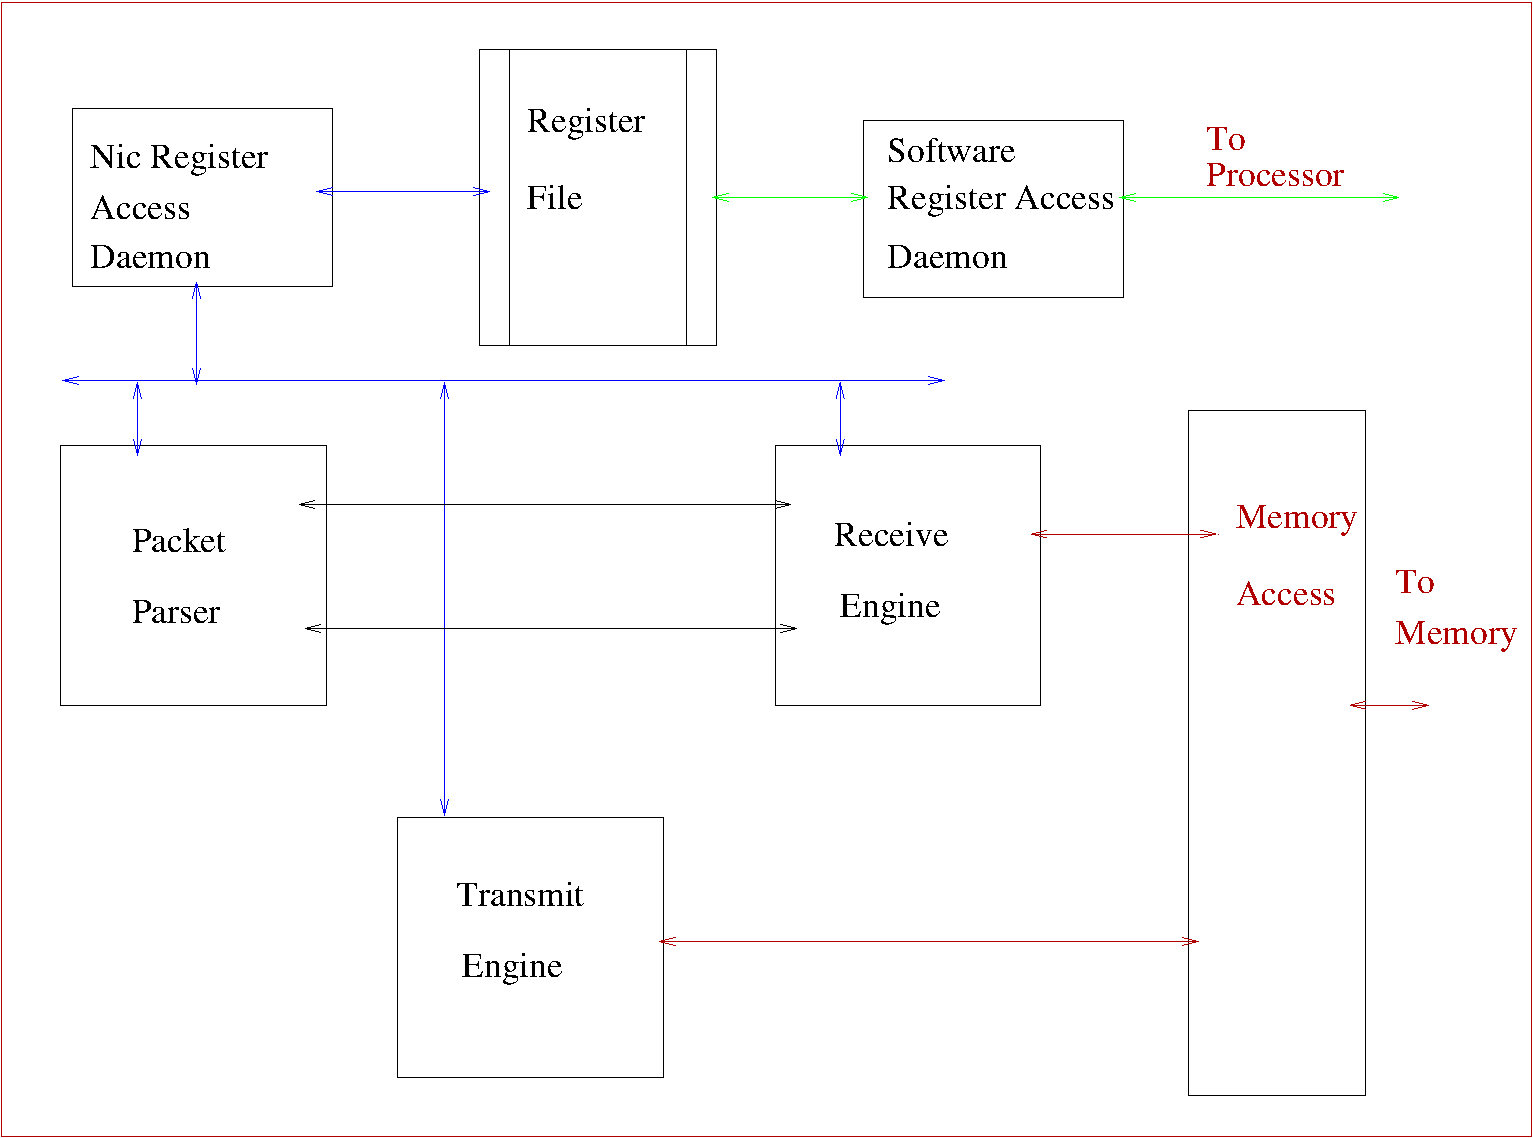
\includegraphics[width=8cm]{./figures/NIC_Internal.pdf}
			\caption{Architecture of Network Interface Controller}
			\label{fig:NIC-Arch}
		\end{figure}

		\subsection{Register File Map} \label{subsec:NIC_REG}
				The NIC (Network Interface Controller) registers are specific memory locations within the NIC that are used for configuration, control, and status monitoring purposes. These registers allow communication between the processor and the NIC, enabling the processor to control and monitor NIC. The NIC registers provide a standardized interface for the processor to interact with the NIC and perform tasks such as enabling or disabling the NIC, setting queue address and monitoring the status of data transmission and reception. See table~\ref{tab:NIC_REG} for description of NIC registers.

			\begin{table}[h!]
				\centering
				\begin{tabular}{|c|c|c|}
					\hline
					Reg. ID& Address offset & Description  \\ \hline
					0  & 0x00  & Control reg    \\ \hline
					1  & 0x04  & Number of Servers    \\ \hline
					2  & 0x08  & Address of rx\_queue    \\ \hline
					10  & 0x28  & Address of tx\_queue    \\ \hline
					18  & 0x48  & Address of free queue    \\ \hline
				\end{tabular}
				\caption{NIC registers map}
				\label{tab:NIC_REG}
			\end{table}


		\subsection{Parser}
				The parser daemon receives data from the MAC (Media Access Control) through a pipe and extracts relevant information from Ethernet packets. It utilizes a state machine to process chunks of data and identifies essential details such as source and destination MAC addresses, type/length field, and packet data. The parsed information is then forwarded to receive engine daemon. The algorithm~\ref{alg:ParserCode} shows psuedo code of parser.

		\subsection{Receive Enigne}
				The receive engine daemon is responsible for the storage of packets coming from the parser. It receives the parsed packet information from the parser daemon and interacts with the processor to ensure the proper handling of received packets. The receive engine daemon uses the free\_queue, to get an empty buffer address to store the active packets in buffers.
			Then uses rx\_queue to provide their(buffer's) addresses to the processor for processing. The algorithm~\ref{alg:RecEnigne} showspsuedo code of receive engine,
		\subsection{Transmit Engine}
				The transmit engine daemon focuses on transmitting processed packets from the processor to the external network. It receives the addresses of processed packet buffers from the processor via the tx\_queue and sends the corresponding packets out through the Ethernet interface. The transmit engine daemon monitors the tx\_queue and retrieves the buffer addresses to facilitate efficient packet transmission. The daemon also pushes free\_queue with the address of buffers which is sent out. This allows the reuse of buffers. The algorithm~\ref{alg:TxEngine} shows psuedo code of transmit engine.
			\subsection{Software register Access}
				The software register access daemon enables the the processor to access and modify the NIC's software registers. These registers contain various control and configuration parameters, allowing the processor to configure and manage the behavior of the NIC. The software register access daemon handles the communication between the processor and the NIC registers, ensuring reliable and secure access. The processor uses AFB protocol(see section ~\ref{AFB}) for register access.\\

	

		\subsection{Nic register Access}
				The NIC register access daemon provides the necessary interface for the NIC to read from and write to its internal registers. These registers store critical information for the proper functioning of the NIC, including configuration settings, status flags, and other control parameters. The NIC register access daemon ensures that the processor can interact with these registers and modify them as needed to configure and manage the NIC's behavior.\\
		\begin{table}[!htbp]
					\centering
					\begin{tabular}{ccl}
						\hline
						\textbf{Signal Name} 			& \textbf{Location} 		&{c}\textbf{Signal Description}  \\ \hline
						\multirow{2}{*}{\textit{read/write\_bar}}& \multirow{2}{*}{[42:42]}	& if `1', the request is read request,\\ 
											& 				& if `0', the request is write request.\\ \hline
						\multirow{3}{*}{\textit{byte\_mask}}	& \multirow{3}{*}{[ 41: 38]}	& \textit{byte\_mask} is 4 bit field, each bit is mapped\\
											&				& to 4 bytes of data. if any bit is `1' then\\
											& 				& corresponding byte in data is valid else not.\\ \hline 
						\multirow{2}{*}{\textit{reg\_index}}   	& \multirow{2}{*}{[37:32]} 	& index of register to which read/write should\\ 
											&				& be performed.\\ \hline
						\textit{write\_data}   			& [31: 0] 			& Data to be written.\\ \hline
					\end{tabular}
					\caption{NIC to Register file interface description}
					\label{tab:NIC-Reg-interface-req}
				\end{table}

				\begin{table}[!htbp]
					\centering
					\begin{tabular}{ccl}
						\hline
						\textbf{Signal Name} 		& \textbf{Location} 		&\textbf{Signal Description}  \\ \hline
						\textit{err}			& [32:32]			& Value `1' indicates errored response.\\\hline
						\textit{data}   		& [31: 0] 			& Contains read data if the req. was read req.\\ \hline
					\end{tabular}
					\caption{ Register file to NIC interface description}
					\label{tab:Reg-NIC-interface-resp}
				\end{table}


		\section{Helper Modules}
			\begin{enumerate}
				\item \textbf{memoryAccess}: This module can be called from other modules and used to read and write from and to memory. 
				\item \textbf{pusiIntoQueue}: This module is used to push buffer pointer to provided queue. 
				\item \textbf{popFromQueue}: This module is used to pop buffer pointer form provided queue. 
				\item \textbf{acquireLock}: This module is used to lock the queue for push and pop operation. It first reads the queue lock by setting memory lock to `1' and then acquires queue lock if its available and then releases memory lock.
				\item \textbf{releaseLock}: This module is used to release the acquired queue lock.
			\end{enumerate}	

 \section{Validation and Performance}
                The data rate found using 1x1x32 (single core single-threaded) AJIT processor are as shown in table~\ref{table_dataRate}. The peak performance achived in this case is 114.81Mbps.
                \begin{table*}[htbp]
                        \caption{Data rate achieved for differnet number of packets \& packet sizes}
                        \begin{center}
                                \begin{tabular}{|c|c|c|c|}
                                        \hline
                                        & \multicolumn{3}{c|}{\textbf{Packet Size}(in Bytes)}\\
                                        \hline
                                        \textbf{No. of Packets}& \textbf{48}                    & \textbf{136}                  & \textbf{236}    \\
                                        \hline
                                        &  \multicolumn{3}{c|}{\textbf{Data Rate}(in Mbps)}\\
                                        \hline
                                        1                       & 11.3316                       & 31.7085                       & 51.2869 \\
                                        \hline
                                        10                      & 18.8431                       & 57.2255                       & 102.4069\\
                                        \hline
                                        100                     & 22.4589                       & 64.1140                       & 110.9845\\
%                                       \hline
%                                       500                     & 22.9792                       & 64.0819                       & 114.2853\\
                                        \hline
                                        1000                    & 23.0982                       & 64.0665                       & 114.4293\\
%                                       \hline
%                                       5000                    & 23.0336                       & 64.3663                       & 114.7432\\
                                        \hline
                                        10000                   & 23.0892                       & 64.3163                       & 114.7907\\
                                        \hline
                                        50000                   & 23.0983                       & 64.4662                       & 114.8123\\
                                        \hline
                                \end{tabular}
                                \label{table_dataRate}
                        \end{center}
                \end{table*}

        To avoid the processor from locking queues the setup was designed where processor will first generate 1750 packets of size 146 bytes, and push them to tx\_queue. NIC will read the tx\_queue and send the packets out during this time. The peak performance achieved is 433.2847 Mbps in this case.
 
 
	 This chapter focused on NIC architecture and interfaces which was then followed by NIC's performance. Now we describe the design and validation of SoC using this NIC and an accelerator in the next chapter.
%Table \ref{table:a} lists out energy, timing, and power values for some of the sensors depicted in \cite{3}:
%\begin{table}[ht]
%\centering % used for centering table
%\begin{tabularx}{\linewidth}{c*{5}{>{\centering\arraybackslash}X}} % centered columns (5 columns)
%\hline\hline %inserts double horizontal lines
% Sensor & Energy per Operation ($mJ$) & Operation Time ($s$) & Sleep Time ($s$) & Average Power ($mW$) \\ [0.5 ex] % inserts table
%\centering Sensor & \multicolumn{1}{p{3cm}}{ \centering Energy per Operation \\ ($mJ$) } & \multicolumn{1}{p{2.5cm}}{\centering Operation Time  \\ ($s$) } & \multicolumn{1}{p{2.5cm}}{\centering Sleep \\Time \\ ($s$) } & \multicolumn{1}{p{2.5cm}}{\centering Average Power  \\ ($mW$) }\\
%heading
%\hline % inserts a single horizontal line
%Tyndall Mote & 3.75 & 0.039 & 60 & 0.117\\ % inserting body of the table
%TI eZ430-RF2500 & 0.114 & 0.0029 & 1 & 0.118 \\
%MicaZ & 7.49 & 0.905 & 59 & 0.186 \\ [1ex] % [1ex] adds vertical space
%\hline %inserts a single line
%\end{tabularx}
%\caption{Energy, Timing and Power demands of sensors} % title of Table
%\label{table:a} % is used to refer to this table in the text
%\end{table}\\

%%%%%%%%%%%%%%%%%%%%%%%%%%%%%%%%%%%%%%%%%%%%%%%%%%%%%%%%%%%%%%%%%%%%%
\newpage
\chapter{SoC Design and Validation} \label{3}
\rule[10pt]{\linewidth}{3pt}
We validate an characterize the performance of the accelerator by integrating it into a System-on-chip (SoC) using AJIT Processor, which provides the accelerator with the commands to operate, and reads back the data. The whole system is also connected to a Network Interface Card, which provides high-speed IO for the quick loading of images into the memory. The architecture of the system is shown in Fig~\ref{fig:SoC}.
\\

The system consists of a 32-bit wide AJIT processor at its core. The processor has an ACB interface through which it interacts with memory and other modules. The AFB interface linked to the Network Interface Controller (NIC) and the 8-engine accelerator cluster is used to transfer configuration information from the processor and relay back status flags to it. The modules are also provided with an ACB interface through which they can access the memory. The memory subsystem consists of a DRAM controller connected to an ACB to UI conversion protocol, which translates memory requests in the ACB bus to DRAM requests, and vice versa for the responses. In addition to the above, the processor has a couple of UART interfaces with which it can communicate with the outside world. Also, the NIC has an interface to connect with the Xilinx MAC IP, using which it can communicate to the host machine via Ethernet, currently configured to run at 100Mbps. 
\\


		\begin{figure}[htbp]
			\centering
			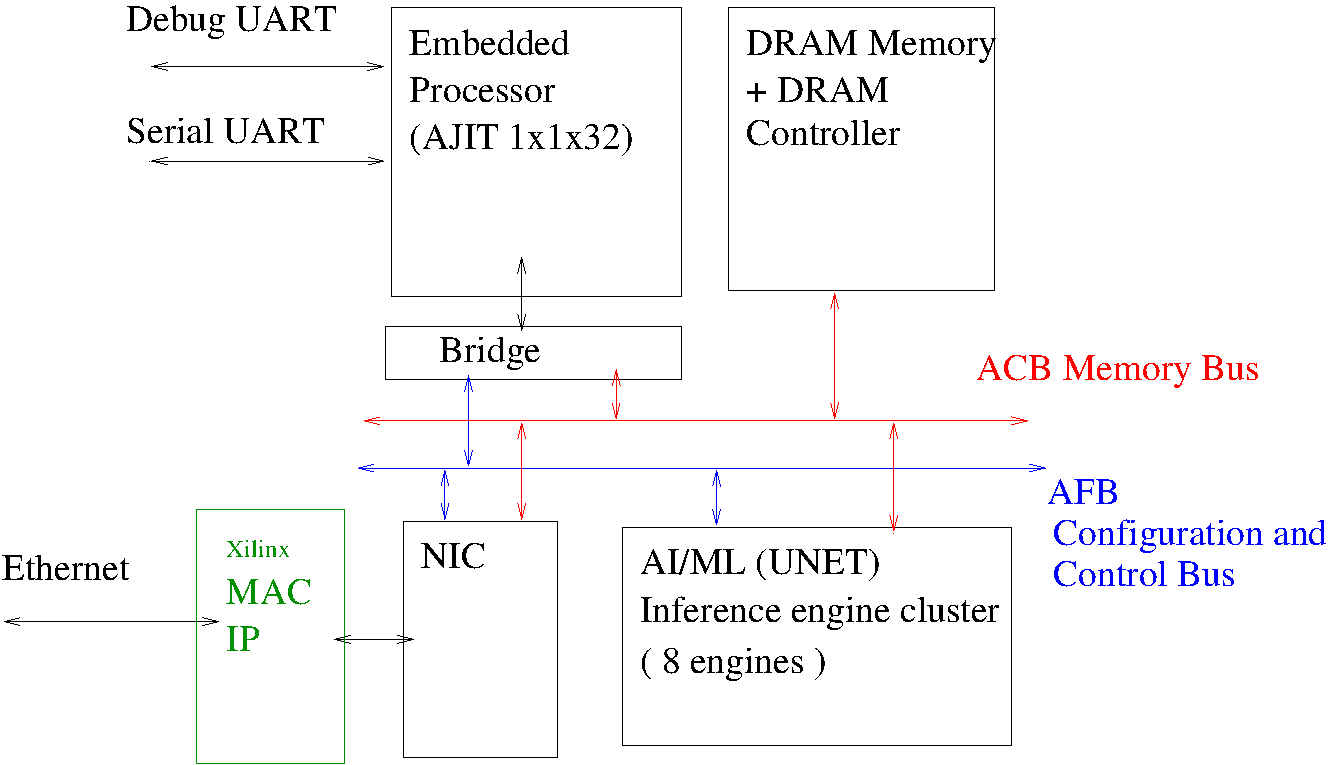
\includegraphics[width=12cm]{./figures/BlockDiagram.pdf}
			\caption{NIC, Processor and accelerator Soc Design}
			\label{fig:SoC}
		\end{figure}

\begin{algorithm}
	\centering
	\begin{verbatim}
	        initialiseMemorySpaces()
	        initialiseNicQueues()
	        fetchKernelsThroughEthernet()
	
	        while(1) do
	                fetchInputsThroughEthernet()
			
	                initliaseAcceleratorStates()
			
	                while (all accelerators not done) do
	                        for engine in list_of_engines do
	                                convolve(engine,stage)
	                                updateState(engine,stage)
	                        end for
	                end while
	                sendOutputsThroughEthernet()
	        end while
	\end{verbatim}
	\caption{The pseudocode for Processor driver}
	\label{alg:ProcAlg}
\end{algorithm}


The above pseudocode shown in algorithm~\ref{alg:ProcAlg} explains the working of the processor code. It first initialise memory spaces required by all modules. These include the queues required by NIC, the kernel addresses for the accelerators and the memory spaces for receiving and storing tensors during computation by the engines. After the memory spaces are initialised, all the queues for NIC are configured and initialised, and the Network Interface Controller starts executing. The kernels are then fetched in through Ethernet, which is then followed by the input tensors for all the engines. With the setup ready, NIC is turned off and the engines are allowed to execute on the data stage by stage. When all the acclerators are done with their computation, the output data is sent to the host PC through Ethernet, where the output is verified for correctness.
\\

The above is a simplified driver to demonstrate the functionality of using multiple accelerator engines inside the system using polling. The processor and the accelerators both support the use of interrupts. The Interrupt Service Routine corresponding to the accelerator interrupts can be suitably configured to allow the processor to be used for other processes, while the engines work on the compute-intensive AI/ML tasks, the completion of which can be signaled to the processor, at which the processor interrupts and schedules the next task to the accelerator before resuming its execution.
\\


\section{Processor NIC Interface}

The processor initializes the queues for the NIC and starts the NIC. When NIC receives data from MAC it pops the free\_queue which has empty packet buffers address stored in it and writes the packet to that buffer. After successfully writing the packet NIC pushes the address of the buffer to rx\_queue, any buffer address in rx\_queue indicates that this is the received packet and needs some action by the processor. While this thing is going on, the processor keeps polling the rx\_queue, as soon as it gets any data over there it reads it and takes the decision. In this setup, the processor is expected to store the packet at some memory location which is shared with the accelerator through its registers. After this packet storage is complete, the processor pushes this address to tx\_queue which works as acknowledgment for the host, after receiving it (the host) sends a new packet. This is the overall flow for storing files in the memory.
\\

Now to send the files out on the ethernet interface the processor breaks a file into a number of packets, pops free\_queue for empty buffer address, and stores the packet at that address. After storing the packet successfully, the processor pushes the buffer address to tx\_queue. The transmit engine running inside NIC which is polling this tx\_queue reads that buffer and sends it out. One by one all the packets are sent out.



\section{Processor Accelerator Interface}

The processor begins by feeding the data to registers 1 to 12. After that, it sets the bits 0 and 2 of register 0, which signals the accelerator to start working. The processor can then continue with other tasks or poll on register 0 as it waits for the accelerator to complete, which is indicated by setting bit 4 of register 0 as high. Then, the processor updates the registers to the parameters for the next stage or image.
\\

In addition, the accelerator has a control daemon that resets the registers, reads the data from the AFB\_ACCELERATOR\_REQUEST, writes them onto the accelerator registers, and sends back the response to the AFB\_ACCELERATOR\_RESPONSE. The control daemon runs infinitely waiting on AFB\_ACCELERATOR\_REQUEST requests from the processor.
\\

The accelerator also has a worker daemon, which waits for the appropriate bits to be set in the r0 register. When the processor sends the request to execute through the registers, it calls the core function with the parameters stored by the processor in other registers. When the execution is completed, it writes back 0 into bit 4 of r0, thereby signaling the processor that the computation is completed.
\\

The accelerator also has an interrupt daemon that waits on bit 4 of r0, and sets the signal ACCELERATOR\_INTERRUPT\_8 corresponding to the above bit. The interrupt signal is not currently used but can be utilized to prevent the processor from polling on r0 while the accelerator performs the computation.
\\

\section{Timing Result and Performance}

	Using the designed drivers the timing and performance is calculated. All the readings are taken for 8 accelerator system. 
	It contains 4 main paramerters, 

	\begin{enumerate}
		\item Initial setup time : Time to send kernels = 4.59 sec
		\item Input time : Time to send input image = 89.4 msec
		\item Output time : Time to receive output image = 94.6 msec
		\item Amortized round trip time per image = 0.42 sec
	\end{enumerate}

	Freames per seconds can be calculated using this Amortized round trip time. The equation~\ref{eqn:fps} shows the calculation for FPS.

	\begin{center}

		\begin{equation}\label{eqn:fps}
				FPS = \frac {1} {\text{Amortized round trip time per image}} = \frac{1}{0.42} = 2.38 fps	
		\end{equation}
	\end{center}

	The size of input image is 224x224x3 Bytes, Time required to send this image can give us data rate. 
	The Data rate achieved using this setup is shown in equation~\ref{eqn:datarate}.

	\begin{center}

		\begin{equation}\label{eqn:datarate}
			\text{Data Rate} = \frac {\text{image size in bits}} {\text{Input Time in sec}} = \frac{224\times224\times3\times8}{89.4} = 13.67 	Mbps
		\end{equation}
	\end{center}


%%%%%%%%%%%%%%%%%%%%%%%%%%%%%%%%%%%%%%%%%%%%%%%%%%%%%%%%%%%%%%%%%%%%%
\newpage
\chapter{Conclusion \& Future Work} \label{4}
\rule[10pt]{\linewidth}{3pt}	

	The research and work shows that NIC is designed successfully using AHIR-V2 tools. Then it is integrated with the AJIT SoC prototype. A successful integration is also done to use NIC to provide inputs and output to the AI/ML accelerator. The design can provide speed upto 114Mbps with processor and 433Mbps alone. Also the design gives 2.38fps rate for the acceleration example.
	
	This performance can further be incereased by adding multiple memory banks in case of accleratior SoC and by having some advnaced packet flow mechanisms. The NIC can act as building block for multiple applications like Router, Switches and other network appliances.
	
	The NIC design can be modified to add intelligence to it so that it can do self routing as well as can apply some security algorithms on packets.

\appendix
\begin{appendices}
\renewcommand{\thechapter}{\Roman{chapter}}

\iffalse
\chapter{}\label{a1}
\begin{lstlisting}[language=Verilog, caption= tmp code template,label={label:1}] 
module sum(
	input a,b;
	output sum, cout
	);

	assign {cout, sum} = a + b;

endmodule
\end{lstlisting}
\fi

	
\chapter{}
	\begin{algorithm}[htbp]
		\centering
		\begin{verbatim}
		typedef struct _CortosQueueHeader {
		        uint32_t totalMsgs; // current total messages
		        uint32_t readIndex;
		        uint32_t writeIndex;
		        uint32_t length;
		        uint32_t msgSizeInBytes;
		        uint8_t *lock;
		        uint8_t *bget_addr;
		        // if misc == 1, then assume single writer 
		        // and single reader and don't use locks
		        uint32_t misc;
		} CortosQueueHeader;
		\end{verbatim}
		\caption{Cortos Queue Header}
		\label{alg:QueueHDR}
	\end{algorithm}



	\begin{algorithm}[htbp]
		\centering
		\begin{verbatim}
			loop1 :
			if(enable_by_processor)
			       loop2 :
			       -> read from MAC
			       -> if(Header) 
			                -> send to header & packet pipe
			                -> goto loop2
			       -> else
			       	        -> send to packet pipe
			       	        -> goto loop2
			else
			       -> goto loop1
		\end{verbatim}
		\caption{Parser pseudo code}
		\label{alg:ParserCode}
	\end{algorithm}


	
	\begin{algorithm}
		\centering
		\begin{verbatim}
			loop1 :
			if(enable_by_processor)
			       loop2 :
			       -> count = 0;
			       -> buf_addr = pop from free queue
			       loop2.1:
			       -> Read from header_pipe and write to buff_addr
			       -> count++
			       -> if(!header_end)
			       	        -> goto loop2.1
			       loop2.2:
			       -> Read from packet pipe and write to buf_addr 
			       -> count++
			       -> if(last_chunk)
			       	        -> write count and last bytemast to buf_addr[0].
			       	        -> push buf_addr to rx_queue.
			                -> goto loop2
			       -> else
			       	        -> goto loop2.2
			else
			       -> goto loop1
		\end{verbatim}
		\caption{Receive engine psuedo code}
		\label{alg:RecEngine}
	\end{algorithm}

\begin{algorithm}
		\centering
		\begin{verbatim}
			loop1 : 
			if(enable_by_processor)
			        loop2:
			        -> buf_addr = try to pop tx_queue
			        -> if(pop successful)
			                -> Rx = read control data(buf_addr[0]) 
			                -> count = extractCountFromRx(Rx)
			                loop3:
			                -> read packet from buf_addr
			                -> send out to MAC
			                -> count--
			                -> if(count == 0)
			                        -> push buf_addr to free_queue.
			                        -> goto loop2 
			                -> else
			                        -> goto loop3
			        -> else
			                        -> goto loop2
			->else
			        goto loop1
		\end{verbatim}
		\caption{Transmit engine psuedo code}
		\label{alg:TxEngine}
	\end{algorithm}

\chapter{}


	Description of Prototype router software designe by Niral Networks.














\iffalse
\begin{algorithm}
\caption{Tmp alg template to use.}\label{alg:cap}
\begin{algorithmic}
\Require $n \geq 0$
\Ensure $y = x^n$
\State $y \gets 1$
\State $X \gets x$
\State $N \gets n$
\While{$N \neq 0$}
\If{$N$ is even}
    \State $X \gets X \times X$
    \State $N \gets \frac{N}{2}$  \Comment{This is a comment}
\ElsIf{$N$ is odd}
    \State $y \gets y \times X$
    \State $N \gets N - 1$
\EndIf
\EndWhile
\end{algorithmic}
\end{algorithm}
\fi
\end{appendices}


%\bibliographystyle{ieee}
%\bibliography{reference}
\clearpage
%\addcontentsline{toc}{chapter}{Bibliography}
%\begin{thebibliography}{99}

%%\bibitem{1} G. Saini and M. Shojaei Baghini, "A Generic Power Management Circuit for Energy Harvesters With Shared Components Between the MPPT and Regulator," in IEEE Transactions on Very Large Scale Integration (VLSI) Systems, vol. 27, no. 3, pp. 535-548, March 2019, doi: 10.1109/TVLSI.2018.2885928. 

%\end{thebibliography}
\end{document}
